\part{Introduction}

JavaScript (JS)\cite{javascript} is an interpreted computer programming language. As part of web browsers, implementations allow client-side scripts to interact with the user, control the browser, communicate asynchronously, and alter the document content that is displayed. It has also become common in server-side programming, game development and the creation of desktop applications.


JavaScript is a prototype-based scripting language with dynamic typing and has first-class functions. Its syntax was influenced by C. JavaScript copies many names and naming conventions from Java, but the two languages are otherwise unrelated and have very different semantics. The key design principles within JavaScript are taken from the Self and Scheme programming languages. It is a multi-paradigm language, supporting object-oriented, imperative, and functional programming styles.


The application of JavaScript to uses outside of web pages~—~for example, in PDF documents, site-specific browsers, and desktop widgets~—~is also significant. Newer and faster JavaScript VMs and frameworks built upon them (notably Node.js) have also increased the popularity of JavaScript for server-side web applications.

JavaScript was formalized in the ECMAScript language standard and is primarily used as part of a web browser (client-side JavaScript). This enables programmatic access to computational objects within a host environment.

JavaScript是一种动态类型、弱类型、基于原型的语言,JavaScript不仅是直译式脚本语言,而且内置支持类型,它的解释器(被称为JavaScript引擎)也是浏览器的一部份。



JavaScript最早是在HTML网页上使用,用来给HTML网页增加动态功能,比如JavaScript 常用于验证用户的输入,比如在下面的例子中,如果输入值不是数字,浏览器会弹出提示框。



\begin{lstlisting}[language=HTML]
<input id="demo" type="text">

<script>
function myFunction()
{
var x=document.getElementById("demo").value;
if(x==""||isNaN(x))
	{
	alert("Not Numeric");
	}
}
</script>

<button type="button" onclick="myFunction()">点击这里</button>
\end{lstlisting}

不同于服务器端脚本语言,例如PHP与ASP,JavaScript主要被作为客户端脚本语言在用户的浏览器上运行,不需要服务器的支持,所以在早期程序员比较青睐于JavaScript以减少对服务器的负担,而与此同时也带来另一个问题:安全性。


然而现在随着服务器的强壮,虽然现在的程序员更喜欢运行于服务端的脚本以保证安全,但JavaScript仍然以其跨平台、容易上手等优势被应用于不同的接口上,而且JavaScript也开始被用于网络服务器,如Node.js。

有些特殊功能(如AJAX)必须依赖Javascript在客户端进行支持。随着引擎如V8和框架如Node.js的发展,及其事件驱动及异步IO等特性,JavaScript逐渐被用来编写服务器端程序。



\chapter{Histroy}

JavaScript was originally developed by Brendan Eich. While battling with Microsoft over the Web, Netscape considered their client-server offering a distributed OS, running a portable version of Sun Microsystems' Java. Because Java was a competitor of C++ and aimed at professional programmers, Netscape also wanted a lightweight interpreted language that would complement Java by appealing to nonprofessional programmers, like Microsoft's Visual Basic.

Although it was developed under the name Mocha, the language was officially called LiveScript when it first shipped in beta releases of Netscape Navigator 2.0 in September 1995, but it was renamed JavaScript when it was deployed in the Netscape browser version 2.0B3.


The change of name from LiveScript to JavaScript roughly coincided with Netscape adding support for Java technology in its Netscape Navigator web browser. The final choice of name caused confusion, giving the impression that the language was a spin-off of the Java programming language, and the choice has been characterized by many as a marketing ploy by Netscape to give JavaScript the cachet of what was then the hot new web programming language.

Netscape introduced an implementation of the language for server-side scripting (SSJS) with Netscape Enterprise Server, first released in December, 1994 (soon after releasing JavaScript for browsers). Since the mid-2000s, there has been a proliferation of server-side JavaScript implementations. Node.js is one recent notable example of server-side JavaScript being used in real-world applications.


JavaScript very quickly gained widespread success as a client-side scripting language for web pages. Microsoft introduced JavaScript support in its own web browser, Internet Explorer, in version 3.0, released in August 1996. Microsoft's webserver, Internet Information Server, introduced support for server-side scripting in JavaScript with release 3.0 (1996). Microsoft started to promote webpage scripting using the umbrella term Dynamic HTML.



Microsoft's JavaScript implementation was later renamed JScript to avoid trademark issues. JScript added new date methods to fix the Y2K-problematic\footnote{Y2K问题则是直接与Java有关。\newline 根据设想,\textsf{Date.getYear()}返回的应该是年份的最后两位,但是实际上,对于2000年,它返回的是100。如果用这个函数生成年份,某些网页可能出现``19100"这样的结果。\newline 这个问题完全来源于Java,因为Javascript的日期类直接采用了\textcolor{Blue}{\texttt{java.util.Date}}函数库。Brendan Eich显然很不满意这个结果,这导致后来不得不添加了一个返回四位数年份的\textsf{Date.getFullYear()}函数。} methods in JavaScript, which were based on Java's \textcolor{Blue}{\texttt{java.util.Date}} class.


In November 1996, Netscape announced that it had submitted JavaScript to Ecma International for consideration as an industry standard, and subsequent work resulted in the standardized version named ECMAScript. In June 1997, Ecma International published the first edition of the ECMA-262 specification. A year later, in June 1998, some modifications were made to adapt it to the ISO/IEC-16262 standard, and the second edition was released. The third edition of ECMA-262 (published on December 1999) is the version most browsers currently use.

A fourth edition of the ECMAScript standard was not released and does not exist. Fifth edition of the Ecmascript standard was released in December 2009. The current edition of the ECMAScript standard is 5.1, released in June 2011.

JavaScript has become one of the most popular programming languages on the web. Initially, however, many professional programmers denigrated the language because its target audience consisted of web authors and other such "amateurs", among other reasons. The advent of Ajax returned JavaScript to the spotlight and brought more professional programming attention. The result was a proliferation of comprehensive frameworks and libraries, improved JavaScript programming practices, and increased usage of JavaScript outside of web browsers, as seen by the proliferation of server-side JavaScript platforms.


In January 2009, the CommonJS project was founded with the goal of specifying a common standard library mainly for JavaScript development outside the browser.

CommonJS is a project with the goal of specifying an ecosystem for JavaScript outside the browser (for example, on the server or for native desktop applications). The project was started by Kevin Dangoor in January 2009 and initially named ServerJS.

In August 2009, the project was renamed CommonJS to show the broader applicability of the APIs. Specifications are created and approved in an open process. A specification is only considered final after it has been finished by multiple implementations. CommonJS is not affiliated with the Ecma International group TC39 working on ECMAScript, but some members of TC39 participate in the project.

Today, ``JavaScript" is a trademark of Oracle Corporation. It is used under license for technology invented and implemented by Netscape Communications and current entities such as the Mozilla Foundation.

大概在 1992 年,一家称作 Nombas 的公司开发了一种叫做 C 减减(C-minus-minus,简称 Cmm)的嵌入式脚本语言。Cmm 背后的理念很简单:一个足够强大可以替代宏操作(macro)的脚本语言,同时保持与 C (和 C ++)足够的相似性,以便开发人员能很快学会。这个脚本语言捆绑在一个叫做 CEnvi 的共享软件中,它首次向开发人员展示了这种语言的威力。

Nombas 最终把 Cmm 的名字改成了 ScriptEase\footnote{原因是后面的部分(mm)听起来过于消极,同时字母 C “令人害怕”。},现在 ScriptEase 已经成为了 Nombas 产品背后的主要驱动力。

当 Netscape Navigator 崭露头角时,Nombas 开发了一个可以嵌入网页中的 CEnvi 的版本。这些早期的试验被称为 Espresso Page(浓咖啡般的页面),它们代表了第一个在万维网上使用的客户端语言。而 Nombas 丝毫没有料到它的理念将会成为万维网的一块重要基石。

当网上冲浪越来越流行时,对于开发客户端脚本的需求也逐渐增大。此时,大部分因特网用户还仅仅通过 28.8 kbit/s 的调制解调器连接到网络,即便这时网页已经不断地变得更大和更复杂。而更加加剧用户痛苦的是,仅仅为了简单的表单有效性验证,就要与服务器进行多次地往返交互。设想一下,用户填完一个表单,点击提交按钮,等待了 30 秒的处理后,看到的却是一条告诉你忘记填写一个必要的字段。

那时正处于技术革新最前沿的 Netscape,开始认真考虑开发一种客户端脚本语言来解决简单的处理问题。

当时工作于 Netscape 的 Brendan Eich,开始着手为即将在 1995 年发行的 Netscape Navigator 2.0 开发一个称之为 LiveScript\footnote{Netscape 与 Sun 及时完成了LiveScript 实现。}的脚本语言,当时的目的是在浏览器和服务器(本来要叫它 LiveWire)端使用它,而且就在 Netscape Navigator 2.0 即将正式发布前,Netscape 将其更名为 JavaScript,目的是为了利用 Java 这个因特网时髦词汇。Netscape 的赌注最终得到回报,JavaScript 从此变成了因特网的必备组件。

在1995年时,JavaScript由Netscape公司的布兰登·艾克,在Netscape浏览器上首次设计实现。因为Netscape公司与Sun公司合作,Netscape公司管理层次结构希望它外观看起来像Java,因此取名为JavaScript,但实际上它的语法风格与Self及Scheme较为接近\footnote{Netscape在最初将其脚本语言命名为LiveScript,后来Netscape在与Sun合作之后将其改名为JavaScript。JavaScript最初受Java启发而开始设计的,目的之一就是“看上去像Java”,因此语法上有类似之处,一些名称和命名规范也借自Java,但JavaScript的主要设计原则源自Self和Scheme。JavaScript与Java名称上的近似,是当时Netscape为了营销考虑与Sun Microsystem达成协议的结果。}。

因为 JavaScript 1.0 如此成功,Netscape 在 Netscape Navigator 3.0 中发布了 1.1 版。恰巧那个时候,微软决定进军浏览器,发布了 IE 3.0 并搭载了一个 JavaScript 的克隆版,叫做 JScript(这样命名是为了避免与 Netscape 潜在的许可纠纷)。微软步入 Web 浏览器领域的这重要一步虽然令其声名狼藉,但也成为 JavaScript 语言发展过程中的重要一步。

在微软进入后,有 3 种不同的 JavaScript 版本同时存在:Netscape Navigator 3.0 中的 JavaScript、IE 中的 JScript以及CEnvi推出的ScriptEase,它们与JavaScript同样都可在浏览器上运行,因此在JavaScript的标准并未确定时,同期有Netscape的JavaScript,微软的JScript和CEnvi的ScriptEase三足鼎立。

与 C 和其他编程语言不同的是,JavaScript 并没有一个标准来统一其语法或特性,而这 3 种不同的版本恰恰突出了这个问题。随着业界担心的增加,这个语言的标准化显然已经势在必行。

\chapter{ECMAScript}

1997 年,JavaScript 1.1 作为一个草案提交给欧洲计算机制造商协会(ECMA)。第 39 技术委员会(TC39)被委派来“标准化一个通用、跨平台、中立于厂商的脚本语言的语法和语义”(\url{http://www.ecma-international.org/memento/TC39.htm})。

为了统一规格,1997年,在ECMA(欧洲计算机制造商协会)的协调下,由来自Netscape、Sun、微软、Borland和其他一些对脚本编程感兴趣的公司的程序员组成的 TC39组成的工作组确定了统一标准:ECMA-262。

ECMA-262标准定义了名为 ECMAScript 的全新脚本语言。因为JavaScript兼容于ECMA标准,因此也称为ECMAScript,符合ECMA-262 3rd Edition标准的实现包括:

\begin{compactitem}
\item Microsoft公司的JScript
\item Mozilla的JavaScript-C(C语言实现),现名SpiderMonkey
\item Mozilla的Rhino(Java实现)
\item Digital Mars公司的DMDScript
\item Google公司的V8
\item WebKit
\end{compactitem}


在接下来的几年里,国际标准化组织及国际电工委员会(ISO/IEC)也采纳 ECMAScript 作为标准(ISO/IEC-16262)。从此,Web 浏览器就开始努力(虽然有着不同的程度的成功和失败)将 ECMAScript 作为 JavaScript 实现的基础。

ECMAScript 分成几个不同的版本,它是在ECMA-262 的标准中定义的。和其他标准一样,ECMA-262 会被编辑和更新。当有了主要更新时,就会发布一个标准的新版。最新 ECMA-262 的版本是 5.1,于 2011 年 6 月发布。


ECMA-262 的第一版在本质上与 Netscape 的 JavaScript 1.1 是一样,只是把所有与浏览器相关的代码删除了,此外还有一些小的调整。首先,ECMA-262 要求对 Unicode 标准的支持(以便支持多语言)。第二,它要求对象是平台无关的(Netscape 的 JavaScript 1.1 事实上有不同的对象实现,例如 Date 对象,是依赖于平台)。这是 JavaScript 1.1 和 1.2 为什么不符合 ECMA-262 规范第一版的主要原因。

ECMA-262 的第二版大部分更新本质上是编辑性的。这次标准的更新是为了与 ISO/IEC-16262 的严格一致,也并没有特别添加、更改和删除内容。ECMAScript 一般不会遵守第二版。

ECMA-262 第三版是该标准第一次真正的更新。它提供了对字符串处理、错误定义和数值输出的更新。同时,它还增加了正则表达式、新的控制语句、try...catch 异常处理的支持,以及一些为使标准国际化而做的小改动。一般来说,它标志着 ECMAScript 成为一种真正的编程语言。

\begin{longtable}{|m{45pt}|m{220pt}|m{100pt}|}
%head
\multicolumn{3}{r}{}
\tabularnewline\hline
版本	&说明	&实现
\endhead
%endhead

%firsthead
\caption{ECMA}\\
\hline
版本	&说明	&实现
\endfirsthead
%endhead

%foot
\multicolumn{3}{r}{}
\endfoot
%endfoot

%lastfoot
\endlastfoot
%endlastfoot
\hline
ECMA v1	&标准化了JavaScript1.1的基本特性,并添加了一些新特性。没有标准化switch语句和正则表达式。	&由Netscape 4.5和IE 4实现。\\
\hline
ECMA v2	&ECMA v1的维护版本,只添加了说明。															&由Netscape 4.5和IE 4实现。\\
\hline
ECMA v3	&标准化了switch语句、异常处理和正则表达式。													&由Mozilla、Netscape 6和IE 5.5实现。\\
\hline
\end{longtable}






含有 JavaScript 1.1 的 Netscape Navigator 3.0 在 1996 年发布。然后,JavaScript 1.1 规范被作为一个新标准的草案被提交给 EMCA。有了 JavaScript 轰动性的流行,Netscape 十分高兴地开始开发 1.2 版。但有一个问题,ECMA 并未接受 Netscape 的草案。在 Netscape Navigator 3.0 发布后不久,微软就发布了 IE 3.0。该版本的 IE 含有 JScript 1.0(微软自己的 JavaScript 实现的名称),原本计划可以与 JavaScript 1.1 相提并论。然后,由于文档不全以及一些不当的重复特性,JScript 1.0 远远没有达到 JavaScript 1.1 的水平。

在 ECMA-262 第一版定稿之前,发布含有 JavaScript 1.2 的 Netscape Navigator 4.0 是在 1997 年,在那年晚些时候,ECMA-262 标准被接受并标准化。因此,JavaScript 1.2 并不和 ECMAScript 的第一版兼容,虽然 ECMAScript 应该基于 JavaScript 1.1。

JScript 的下一步是 IE 4.0 中加入的 JScript 3.0(2.0 版是随 IIS 3.0 一起发布的,但并未包含在浏览器中)。微软大力宣传 JScript 3.0 是世界上第一个真正符合 ECMA 标准的脚本语言。而那时,ECMA-262 还没有最终定稿,所以 JScript 3.0 也遭受了和 JavaScript 1.2 同样的命运 - 它还是没能符合最终的 ECMAScript 标准。

Netscape 选择在 Netscape Navigator 4.06 中升级它的 JavaScript 实现。JavaScript 1.3 使 Netscape 终于完全符合了 ECMAScript 第一版。Netscape 加入了对 Unicode 标准的支持,并让所有的对象保留了在 JavaScript 1.2 中引入的新特性的同时实现了平台独立。

当 Netscape 将它的源代码作为 Mozilla 项目公布于众时,本来计划 JavaScript 1.4 将会嵌入到 Netscape Navigator 5.0 中。然而,一个冒进的决定——要完全从头重新设计 Netscape 的代码,破坏了这个工作。JavaScript 1.4 仅仅作为一个 Netscape Enterprise Server 的服务器端脚本语言发布,以后也没有被放入浏览器中。

如今,所有主流的 Web 浏览器都遵守 ECMA-262 第三版。下面的表格列出了大部分流行的 Web 浏览器中的 ECMAScript 支持:

\begin{longtable}{|m{150pt}|m{150pt}|}
%head
\multicolumn{2}{r}{}
\tabularnewline\hline
浏览器	&DOM 兼容性
\endhead
%endhead

%firsthead
\hline
浏览器	&DOM 兼容性
\endfirsthead
%endfirsthead

%foot
\multicolumn{2}{r}{}
\endfoot
%endfoot

%lastfoot
\endlastfoot
%endlastfoot

\hline
Netscape Navigator 2.0			&-\\
\hline
Netscape Navigator 3.0			&-\\
\hline
Netscape Navigator 4.0 - 4.05	&-\\
\hline
Netscape Navigator 4.06 - 4.79	&Edition 1\\
\hline
Netscape 6.0+ (Mozilla 0.6.0+)	&Edition 3\\
\hline
Internet Explorer 3.0			&-\\
\hline
Internet Explorer 4.0			&-\\
\hline
Internet Explorer 5.0			&Edition 1\\
\hline
Internet Explorer 5.5+			&Edition 3\\
\hline
Opera 6.0 - 7.1					&Edition 2\\
\hline
Opera 7.2+						&Edition 3\\
\hline
Safari 1.0+/Konqueror~2.0+	&Edition 3\\
\hline
\end{longtable}

\chapter{DOM}



自从 IE 4.0 和 Netscape Navigator 4.0 开始支持不同形态的动态 HTML(DHTML),开发者首次能够在不重载网页的情况下修改它的外观和内容。这是 Web 技术的一大飞跃,不过也带来了巨大的问题。Netscape 和微软各自开发自己的 DHTML,从而结束了 Web 开发者只编写一个 HTML 页面就可以在所有浏览器中访问的时期。

业界决定必须要做点什么以保持 Web 的跨平台特性,他们担心如果放任 Netscape 和微软公司这样做,Web 必将分化为两个独立的部分,每一部分只适用于特定的浏览器。因此,负责指定 Web 通信标准的团体 W3C(World Wide Web Consortium)就开始制定 DOM\footnote{注意,DOM 不是 JavaScript 专有的,事实上许多其他语言都实现了它。不过,Web 浏览器中的 DOM 已经用 ECMAScript 实现了,现在是 JavaScript 语言的一个很大组成部分。}。

DOM(文档对象模型)是 HTML 和 XML 的应用程序接口(API)。DOM 将把整个页面规划成由节点层级构成的文档。HTML 或 XML 页面的每个部分都是一个节点的衍生物。考虑下面的 HTML 页面:


\begin{lstlisting}[language=HTML]
<html>
  <head>
    <title>Sample Page</title>
  </head>
  <body>
    <p>hello world!</p>
  </body>
</html>
\end{lstlisting}

这段代码可以用 DOM 绘制成一个节点层次图:


\begin{figure}[!h]
\centering
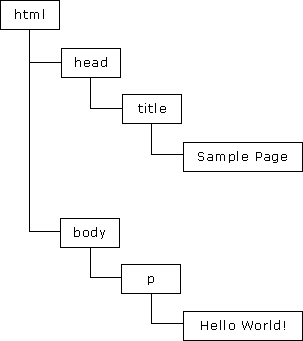
\includegraphics[scale=0.5]{js_dom.png}
\vspace{-10pt}
\caption{DOM节点层次图}
\label{js_dom}
\end{figure}

DOM 通过创建树来表示文档,从而使开发者对文档的内容和结构具有空前的控制力,使用 DOM API 可以轻松地删除、添加和替换节点。

DOM Level 1 是 W3C 于 1998 年 10 月提出的,它由两个模块组成,即 DOM Core 和 DOM HTML。前者提供了基于 XML 的文档的结构图,以便访问和操作文档的任意部分;后者添加了一些 HTML 专用的对象和方法,从而扩展了 DOM Core。

DOM Level 1 只是一个目标,即规划文档的结构,DOM Level 2 的目标就广泛多了。对原始 DOM 的扩展添加了对鼠标和用户界面事件(DHTML 对此有丰富的支持)、范围、遍历(重复执行 DOM 文档的方法)的支持,并通过对象接口添加了对 CSS(层叠样式表)的支持。由 Level 1 引入的原始 DOM Core 也加入了对 XML 命名空间的支持。

DOM Level 2 引入了几种 DOM 新模块,用于处理新的接口类型:

\begin{compactitem}
\item DOM 视图 - 描述跟踪文档的各种视图(即 CSS 样式化之前和 CSS 样式化之后的文档)
\item DOM 事件 - 描述事件的接口
\item DOM 样式 - 描述处理基于 CSS 样式的接口
\item DOM 遍历和范围 - 描述遍历和操作文档树的接口
\end{compactitem}

DOM Level 3 引入了以统一的方式载入和保持文档的方法(包含在新模块 DOM Load and Save)以及验证文档(DOM Validation)的方法,从而进一步扩展了 DOM。在 Level 3 中,DOM Core 被扩展为支持所有的 XML 1.0 特性,包括 XML Infoset、XPath 和 XML Base。

注意,根本没有 DOM Level 0 这个标准,它只是 DOM 的一个历史参考点(DOM Level 0 指的是 IE 4.0 和 Netscape Navigator 4.0 中支持的原始 DHTML)。

除了 DOM Core 和 DOM HTML 外,还有其他几种语言发布了自己的 DOM 标准。这些语言都是基于 XML 的,每种 DOM 都给对应语言添加了特有的方法和接口:

\begin{compactitem}
\item 可缩放矢量语言(SVG)1.0
\item 数字标记语言(MathML)1.0
\item 同步多媒体集成语言(SMIL)
\end{compactitem}

此外,其他语言也开发了自己的 DOM 实现,如 Mozilla 的 XML 用户界面语言(XUL)。不过,只有上面列出的几种语言是 W3C 的推荐标准。

DOM 在被 Web 浏览器开始实现之前就已经是一种标准了。IE 首次尝试 DOM 是在 5.0 版本中,不过其实直到 5.5 版本之后才具有真正的 DOM 支持,IE 5.5 实现了 DOM Level 1。从那时起,IE 就没有引入新的 DOM 功能。

Netscape 直到 Netscape 6(Mozilla 0.6.0)才引入 DOM 支持。目前,Mozilla 具有最好的 DOM 支持,实现了完整的 Level 1、几乎所有 Level 2 以及一部分 Level 3。(Mozilla 开发小组的目标是构造一个与标准 100\% 兼容的浏览器,他们的工作得到了回报。)

Opera 直到 7.0 版本才加入 DOM 支持,还有 Safari 也实现了大部分 DOM Level 1。它们几乎都与 IE 5.5 处于同一水平,有些情况下,甚至超过了 IE 5.5。不过,就对 DOM 的支持而论,所有浏览器都远远落后于 Mozilla。下表列出了常用浏览器对 DOM 的支持。

\begin{longtable}{|m{150pt}|m{180pt}|}
%head
\multicolumn{2}{r}{}
\tabularnewline\hline
浏览器	&DOM 兼容性
\endhead
%endhead

%firsthead
\hline
浏览器	&DOM 兼容性
\endfirsthead
%endfirsthead

%foot
\multicolumn{2}{r}{}
\endfoot
%endfoot

%lastfoot
\endlastfoot
%endlastfoot

\hline
Netscape Navigator 1.0 - 4.x			&-\\
\hline
Netscape 6.0+ (Mozilla 0.6.0+)			&Level 1、Level 2、Level 3(部分)\\
\hline
IE 2.0 - 4.x								&-\\
\hline
IE 5.0									&Level 1(最小)\\
\hline
IE 5.5+									&Level 1(几乎全部)\\
\hline
Opera 1.0 - 6.0							&-\\
\hline
Opera 7.0+								&Level 1(几乎全部)、Level 2 (部分)\\
\hline
Safari 1.0+/Konqueror ~ 2.0+			&Level 1\\
\hline
\end{longtable}


\chapter{BOM}

IE 3.0 和 Netscape Navigator 3.0 提供了一种特性 - BOM(浏览器对象模型),可以对浏览器窗口进行访问和操作。使用 BOM,开发者可以移动窗口、改变状态栏中的文本以及执行其他与页面内容不直接相关的动作。使 BOM 独树一帜且又常常令人怀疑的地方在于,它只是 JavaScript 的一个部分,没有任何相关的标准。

BOM 主要处理浏览器窗口和框架,不过通常浏览器特定的 JavaScript 扩展都被看做 BOM 的一部分。这些扩展包括:

\begin{compactitem}
\item 弹出新的浏览器窗口
\item 移动、关闭浏览器窗口以及调整窗口大小
\item 提供 Web 浏览器详细信息的定位对象
\item 提供用户屏幕分辨率详细信息的屏幕对象
\item 对 cookie 的支持
\item IE 扩展了 BOM,加入了 ActiveXObject 类,可以通过 JavaScript 实例化 ActiveX 对象
\end{compactitem}

由于没有相关的 BOM 标准,每种浏览器都有自己的 BOM 实现。有一些事实上的标准,如具有一个窗口对象和一个导航对象,不过每种浏览器可以为这些对象或其他对象定义自己的属性和方法。



\chapter{Validation}



\section{Form validation}

JavaScript 可用来在数据被送往服务器前对 HTML 表单中的这些输入数据进行验证。

被 JavaScript 验证的这些典型的表单数据有:

\begin{compactitem}
\item 用户是否已填写表单中的必填项目?
\item 用户输入的邮件地址是否合法?
\item 用户是否已输入合法的日期?
\item 用户是否在数据域 (numeric field) 中输入了文本?
\end{compactitem}

下面的函数用来检查用户是否已填写表单中的必填(或必选)项目。假如必填或必选项为空,那么警告框会弹出,并且函数的返回值为 false,否则函数的返回值则为 true(意味着数据没有问题):

\begin{lstlisting}[language=JavaScript]
function validate_required(field,alerttxt){
  with (field)
  {
    if (value==null||value==""){
      alert(alerttxt);
      return false;
    }
    else {
      return true;
    }
  }
}
\end{lstlisting}

下面是连同 HTML 表单的代码:


\begin{lstlisting}[language=HTML]
<html>
<head>
<script type="text/javascript">

function validate_required(field,alerttxt)
{
with (field)
  {
  if (value==null||value=="")
    {alert(alerttxt);return false}
  else {return true}
  }
}

function validate_form(thisform)
{
with (thisform)
  {
  if (validate_required(email,"Email must be filled out!")==false)
    {email.focus();return false}
  }
}
</script>
</head>

<body>
<form action="submitpage.htm" onsubmit="return validate_form(this)" method="post">
Email: <input type="text" name="email" size="30">
<input type="submit" value="Submit"> 
</form>
</body>

</html>
\end{lstlisting}

\section{Email validation}


下面的函数检查输入的数据是否符合电子邮件地址的基本语法。

这里要验证的是,输入的数据必须包含 @ 符号和点号(.)。同时,@ 不可以是邮件地址的首字符,并且 @ 之后需有至少一个点号:

\begin{lstlisting}[language=JavaScript]
function validate_email(field,alerttxt){
  with (field)
  {
    apos=value.indexOf("@")
    dotpos=value.lastIndexOf(".")
    if (apos<1||dotpos-apos<2){
      alert(alerttxt);return false
    }
    else {
      return true
    }
  }
}
\end{lstlisting}

下面是连同 HTML 表单的完整代码:

\begin{lstlisting}[language=HTML]
<html>
<head>
<script type="text/javascript">
function validate_email(field,alerttxt){
  with (field){
    apos=value.indexOf("@")
    dotpos=value.lastIndexOf(".")
    if (apos<1||dotpos-apos<2){
      alert(alerttxt); 
      return false;
    }
    else {
      return true;
    }
  }
}

function validate_form(thisform){
  with (thisform){
    if (validate_email(email,"Not a valid e-mail address!")==false){
      email.focus();
      return false;
    }
  }
}
</script>
</head>

<body>
<form action="submitpage.htm"onsubmit="return validate_form(this);" method="post">
Email: <input type="text" name="email" size="30">
<input type="submit" value="Submit"> 
</form>
</body>

</html>
\end{lstlisting}

\chapter{Features}

Javascript被归类为直译语言,因为目前主流的引擎都是每次运行时加载代码并解译。V8是将所有代码解译后再开始运行,其他引擎则是逐行解译(SpiderMonkey会将解译过的指令暂存,以提高性能,称为实时编译),但由于V8的核心部份多数用Javascript撰写(而SpiderMonkey是用C++),因此在不同的测试上,两者性能互有优劣。

JavaScript作为一种脚本语言,其源代码在发往客户端运行之前不需经过编译,而是将文本格式的字符代码发送给浏览器由浏览器解释运行。直译语言的弱点是安全性较差,而且在JavaScript中,如果一条运行不了,那么下面的语言也无法运行。而其解决办法就是于使用~\textcolor{Blue}{\texttt{try\{\}...catch()\{\}}}︰

\begin{lstlisting}[language=JavaScript]
console.log("a");    //这是正确的
console.log("b");    //这是正确的
console.logg("c");   //这是错误的,并且到这里会停下来
console.log("d");    //这是正确的
console.log("e");    //这是正确的
 
/*解决办法*/
try{console.log("a");}catch(e){}    //这是正确的
try{console.log("b");}catch(e){}    //这是正确的
try{console.logg("c");}catch(e){}   //这是错误的,但是到这里不会停下来,而是跳过
try{console.log("d");}catch(e){}    //这是正确的
try{console.log("e");}catch(e){}    //这是正确的
\end{lstlisting}

与脚本语言相对应的是编译语言,例如C语言,以编译语言编写的程序在运行之前,必须经过编译,将代码编译为机器码,再加以运行。





尽管JavaScript作为给非程序人员的脚本语言,而非作为给程序人员的脚本语言来推广和宣传,但是JavaScript具有非常丰富的特性。例如,JavaScript 能够直接写入 HTML 输出流中:

\begin{lstlisting}[language=JavaScript]
document.write("<h1>This is a heading</h1>");
document.write("<p>This is a paragraph</p>");
\end{lstlisting}

使用 JavaScript 来处理 HTML 内容是非常强大的功能,注意只能在 HTML 输出中使用\texttt{document.write},如果在文档加载后使用该方法(比如在函数中)就会覆盖整个文档。

DOM(文档对象模型)是用以访问 HTML 元素的正式 W3C 标准,JavaScript 能够改变任意 HTML 元素的大多数属性,比如图像、样式等。

类似\texttt{document.getElementByID("some id")}的方法是 HTML DOM 中定义的。

\begin{lstlisting}[language=HTML]
<p id="demo">JavaScript 能改变 HTML 元素的内容。</p>

<script>
function myFunction(){
  x=document.getElementById("demo")  //查找元素
  x.innerHTML="Hello JavaScript";    //改变内容
  x.style.color="#ff0000";           //改变样式
}
</script>

<button type="button" onclick="myFunction()">点击</button>
\end{lstlisting}



JavaScript 能够对事件作出反应,比如对按钮的点击:
\begin{lstlisting}[language=HTML]
<button type="button" onclick="alert('Welcome!')">Click button.</button>

<script>
function changeImage()
{
element=document.getElementById('myimage')
if (element.src.match("bulbon"))
  {
  element.src="bulboff.gif";
  }
else
  {
  element.src="bulbon.gif";
  }
}
</script>

<img id="myimage" onclick="changeImage()" src="bulboff.gif">
\end{lstlisting}

其中,\textcolor{Red}{\texttt{alert()}}函数在 JavaScript 中并不常用,但它对于代码测试非常方便。




因此,JavaScript的基本特点可以概括如下:

\begin{compactitem}
\item 是一种解释性脚本语言(代码不进行预编译)。
\item 主要用来向HTML页面添加交互行为。
\item 可以直接嵌入HTML页面,但写成单独的js文件有利于结构和行为的分离。
\end{compactitem}




The following features are common to all conforming ECMAScript implementations, unless explicitly specified otherwise.


\section{Imperative and structured}


JavaScript supports much of the structured programming syntax from C (e.g., \texttt{if} statements, \texttt{while} loops, \texttt{switch} statements, etc.). One partial exception is scoping: C-style block scoping is not supported. Instead, JavaScript has function scoping (although, block scoping using the \texttt{let} keyword was added in JavaScript 1.7). Like C, JavaScript makes a distinction between expressions and statements. One syntactic difference from C is automatic semicolon insertion, in which the semicolons that terminate statements can be omitted.





\section{Dynamic}


\subsection{Dynamtic typing}

As in most scripting languages, types are associated with values, not with variables. For example, a variable \texttt{x} could be bound to a number, then later rebound to a string. JavaScript supports various ways to test the type of an object, including duck typing.

\begin{lstlisting}[language=Python]
$ python
Type "help", "copyright", "credits" or "license" for more information.
>>> i
Traceback (most recent call last):
  File "<stdin>", line 1, in <module>
NameError: name 'i' is not defined
>>> i = 1
>>> i = "5"
>>> print i
5
>>> i = 1 + "5"
Traceback (most recent call last):
  File "<stdin>", line 1, in <module>
TypeError: unsupported operand type(s) for +: 'int' and 'str'
>>> i 
'5'
\end{lstlisting}



\subsection{Object based}

JavaScript is almost entirely object-based. JavaScript objects are associative arrays, augmented with prototypes. Object property names are string keys. They support two equivalent syntaxes: dot notation (\texttt{obj.x = 10}) and bracket notation (\texttt{obj['x'] = 10}). Properties and their values can be added, changed, or deleted at run-time. Most properties of an object (and those on its prototype inheritance chain) can be enumerated using a \texttt{for...}in loop. JavaScript has a small number of built-in objects such as \texttt{Function} and \texttt{Date}.



\subsection{Run-time evaluation}


JavaScript includes an \texttt{eval} function that can execute statements provided as strings at run-time.

\begin{lstlisting}[language=JavaScript]
<script>
s = "alert('hello')";
eval(s);
</script>
\end{lstlisting}


\section{Functional}


\subsection{First-class functions}

Functions are first-class; they are objects themselves. As such, they have properties and methods, such as \texttt{.call()} and \texttt{.bind()}. A nested function is a function defined within another function. It is created each time the outer function is invoked. In addition, each created function forms a lexical closure: the lexical scope of the outer function, including any constants, local variables and argument values, becomes part of the internal state of each inner function object, even after execution of the outer function concludes.






\section{Prototype-based}



\subsection{Prototypes}

JavaScript uses prototypes where many other object oriented languages use classes for inheritance. It is possible to simulate many class-based features with prototypes in JavaScript.


\subsection{Functions as object constructors}


Functions double as object constructors along with their typical role. Prefixing a function call with \texttt{new} will create an instance of a prototype, inheriting properties and methods from the constructor (including properties from the \texttt{Object} prototype). ECMAScript 5 offers the \texttt{Object.create} method, allowing explicit creation of an instance without automatically inheriting from the \texttt{Object} prototype (older environments can assign the prototype to \texttt{null}). The constructor's \texttt{prototype} property determines the object used for the new object's internal prototype. New methods can be added by modifying the prototype of the object used as a constructor. JavaScript's built-in constructors, such as \texttt{Array} or \texttt{Object}, also have prototypes that can be modified. While it is possible to modify the \texttt{Object} prototype, it is generally considered bad practice because most objects in Javascript will inherit methods and properties from the \texttt{Object} prototype and they may not expect the prototype to be modified.


\subsection{Functions as methods}

Unlike many object-oriented languages, there is no distinction between a function definition and a method definition. Rather, the distinction occurs during function calling; when a function is called as a method of an object, the function's local \texttt{this} keyword is bound to that object for that invocation.



\section{Implicit and Explicit Delegation}



JavaScript is a Delegation Language.



\subsection{Functions as Roles (Traits and Mixins)}


JavaScript natively supports various function based implementations of Role patterns like Traits and Mixins. Such a function defines additional behavior by at least one method bound to the \texttt{this} keyword within its \texttt{function} body. A Role then has to be delegated explicitly via \texttt{call} or \texttt{apply} to objects that need to feature additional behavior that is not shared via the prototype chain.



\subsection{Type Composition and Inheritance}



Whereas explicit function based delegation does cover composition in JavaScript, implicit delegation already happens every time the prototype chain is walked in order to e.g. find a method that might be related to but is not directly owned by an object. Once the method was found it gets called within this objects context. Thus inheritance in JavaScript is covered by a delegation automatism that is bound to the prototype slot of constructor functions.



\section{Miscellaneous}



\subsection{Run-time environment}

JavaScript typically relies on a run-time environment (e.g. a web browser) to provide objects and methods by which scripts can interact with the environment (e.g. a webpage DOM). It also relies on the run-time environment to provide the ability to include/import scripts (e.g. HTML \texttt{<script>} elements). This is not a language feature per se, but it is common in most JavaScript implementations.


\subsection{Variadic functions}


An indefinite number of parameters can be passed to a function. The function can access them through formal parameters and also through the local \texttt{arguments} object. Variadic functions can also be created by using the \texttt{apply} method.



\subsection{Array and object literals}

Like many scripting languages, arrays and objects (associative arrays in other languages) can each be created with a succinct shortcut syntax. In fact, these literals form the basis of the JSON data format.


\subsection{Regular expressions}


JavaScript also supports regular expressions in a manner similar to Perl, which provide a concise and powerful syntax for text manipulation that is more sophisticated than the built-in string functions.




\section{Vendor-specific extensions}


JavaScript is officially managed by Mozilla Foundation, and new language features are added periodically. However, only some JavaScript engines support these new features:


\begin{compactitem}
\item property getter and setter functions (supported by WebKit, Opera, ActionScript, and Rhino)
\item conditional \texttt{catch} clauses
\item iterator protocol (adopted from Python)
\item shallow generators-coroutines (adopted from Python)
\item array comprehensions and generator expressions (adopted from Python)
\item proper block scope via the \texttt{let} keyword
\item array and object destructuring (limited form of pattern matching)
\item concise function expressions (\texttt{function(args)} expr)
\item ECMAScript for XML (E4X), an extension that adds native XML support to ECMAScript
\end{compactitem}






\chapter{Syntax}


\section{Simple examples}


Variables in JavaScript can be defined using the \texttt{var} keyword:

\begin{lstlisting}[language=JavaScript]
var x; //defines the variable x, although no value is assigned to it by default
var y = 2; //defines the variable y and assigns the value of 2 to it
\end{lstlisting}

Note the comments in the example above, both of which were preceded with two forward slashes.

There is no built-in I/O functionality in JavaScript; the runtime environment provides that. The ECMAScript specification in edition 5.1 mentions:

\fbox{
	\parbox[c][30pt][c]{360pt}{
	``... indeed, there are no provisions in this specification for input of external data or output of computed results.''
	}
}

However, most runtime environments have a \texttt{console} object that can be used to print output. Here is a minimalist Hello World program:



\begin{lstlisting}[language=JavaScript]
console.log("Hello world!");
\end{lstlisting}

A simple recursive function:



\begin{lstlisting}[language=JavaScript]
function factorial(n) {
    if (n === 0) {
        return 1;
    }
    return n * factorial(n - 1);
}
\end{lstlisting}

Anonymous function (or lambda) syntax and closure example:




\begin{lstlisting}[language=JavaScript]
var displayClosure = function() {
    var count = 0;
    return function () {
        return ++count;
    };
}
var inc = displayClosure();
inc(); // returns 1
inc(); // returns 2
inc(); // returns 3
\end{lstlisting}

Variadic function demonstration (\texttt{arguments} is a special variable).


\begin{lstlisting}[language=JavaScript]
var sum = function() {
    var i, x = 0;
    for (i = 0; i < arguments.length; ++i) {
        x += arguments[i];
    }
    return x;
}
sum(1, 2, 3); // returns 6
\end{lstlisting}

Immediately-invoked function expressions allow functions to pass around variables under their own closures.

\begin{lstlisting}[language=JavaScript]
var v;
v = 1;
var getValue = (function(v) {
  return function() {return v;};
})(v);
 
v = 2;
 
getValue(); // 1
\end{lstlisting}

\section{More advanced examples}

This sample code displays various JavaScript features.



\begin{lstlisting}[language=JavaScript]
/* Finds the lowest common multiple (LCM) of two numbers */
function LCMCalculator(x, y) { // constructor function
    var checkInt = function (x) { // inner function
        if (x % 1 !== 0) {
            throw new TypeError(x + " is not an integer"); // throw an exception
        }
        return x;
    };
    this.a = checkInt(x)
    //   semicolons   ^^^^  are optional, a newline is enough
    this.b = checkInt(y);
}
// The prototype of object instances created by a constructor is
// that constructor's "prototype" property.
LCMCalculator.prototype = { // object literal
    constructor: LCMCalculator, // when reassigning a prototype, set the constructor property appropriately
    gcd: function () { // method that calculates the greatest common divisor
        // Euclidean algorithm:
        var a = Math.abs(this.a), b = Math.abs(this.b), t;
        if (a < b) {
            // swap variables
            t = b;
            b = a;
            a = t;
        }
        while (b !== 0) {
            t = b;
            b = a % b;
            a = t;
        }
        // Only need to calculate GCD once, so "redefine" this method.
        // (Actually not redefinition—it's defined on the instance itself,
        // so that this.gcd refers to this "redefinition" instead of LCMCalculator.prototype.gcd.)
        // Also, 'gcd' === "gcd", this['gcd'] === this.gcd
        this['gcd'] = function () {
            return a;
        };
        return a;
    },
    // Object property names can be specified by strings delimited by double (") or single (') quotes.
    "lcm" : function () {
        // Variable names don't collide with object properties, e.g. |lcm| is not |this.lcm|.
        // not using |this.a * this.b| to avoid FP precision issues
        var lcm = this.a / this.gcd() * this.b;
        // Only need to calculate lcm once, so "redefine" this method.
        this.lcm = function () {
            return lcm;
        };
        return lcm;
    },
    toString: function () {
        return "LCMCalculator: a = " + this.a + ", b = " + this.b;
    }
};
 
// Define generic output function; this implementation only works for web browsers
function output(x) {
    document.body.appendChild(document.createTextNode(x));
    document.body.appendChild(document.createElement('br'));
}
 
// Note: Array's map() and forEach() are defined in JavaScript 1.6.
// They are used here to demonstrate JavaScript's inherent functional nature.
[[25, 55], [21, 56], [22, 58], [28, 56]].map(function (pair) { // array literal + mapping function
    return new LCMCalculator(pair[0], pair[1]);
}).sort(function (a, b) { // sort with this comparative function
    return a.lcm() - b.lcm();
}).forEach(function (obj) {
    output(obj + ", gcd = " + obj.gcd() + ", lcm = " + obj.lcm());
});
\end{lstlisting}

The following output should be displayed in the browser window.


\begin{lstlisting}[language=JavaScript]
LCMCalculator: a = 28, b = 56, gcd = 28, lcm = 56
LCMCalculator: a = 21, b = 56, gcd = 7, lcm = 168
LCMCalculator: a = 25, b = 55, gcd = 5, lcm = 275
LCMCalculator: a = 22, b = 58, gcd = 2, lcm = 638
\end{lstlisting}


\chapter{Used in web pages}

The most common use of JavaScript is to write functions that are embedded in or included from HTML pages and that interact with the Document Object Model (DOM) of the page. Some simple examples of this usage are:


\begin{compactitem}
\item Loading new page content or submitting data to the server via AJAX without reloading the page (for example, a social network might allow the user to post status updates without leaving the page)
\item Animation of page elements, fading them in and out, resizing them, moving them, etc.
\item Interactive content, for example games, and playing audio and video
\item Validating input values of a web form to make sure that they are acceptable before being submitted to the server.
\item Transmitting information about the user's reading habits and browsing activities to various websites. Web pages frequently do this for web analytics, ad tracking, personalization or other purposes.
\end{compactitem}

JavaScript常用来完成以下任务:

\begin{compactitem}
\item 嵌入动态文本于HTML页面
\item 对浏览器事件作出响应
\item 读写HTML元素
\item 在数据被提交到服务器之前验证数据
\item 检测访客的浏览器信息
\item 控制cookies,包括创建和修改等
\end{compactitem}




Because JavaScript code can run locally in a user's browser (rather than on a remote server), the browser can respond to user actions quickly, making an application more responsive. Furthermore, JavaScript code can detect user actions which HTML alone cannot, such as individual keystrokes. Applications such as Gmail take advantage of this: much of the user-interface logic is written in JavaScript, and JavaScript dispatches requests for information (such as the content of an e-mail message) to the server. The wider trend of Ajax programming similarly exploits this strength.


A JavaScript engine (also known as JavaScript interpreter or JavaScript implementation) is an interpreter that interprets JavaScript source code and executes the script accordingly. The first JavaScript engine was created by Brendan Eich at Netscape Communications Corporation, for the Netscape Navigator web browser. The engine, code-named SpiderMonkey, is implemented in C. It has since been updated (in JavaScript 1.5) to conform to ECMA-262 Edition 3. The Rhino engine, created primarily by Norris Boyd (formerly of Netscape; now at Google) is a JavaScript implementation in Java. Rhino, like SpiderMonkey, is ECMA-262 Edition 3 compliant.


A web browser is by far the most common host environment for JavaScript. Web browsers typically create "host objects" to represent the Document Object Model (DOM) in JavaScript. The web server is another common host environment. A JavaScript webserver would typically expose host objects representing HTTP request and response objects, which a JavaScript program could then interrogate and manipulate to dynamically generate web pages.


Because JavaScript is the only language that the most popular browsers share support for, it has become a target language for many frameworks in other languages, even though JavaScript was never intended to be such a language. Despite the performance limitations inherent to its dynamic nature, the increasing speed of JavaScript engines has made the language a surprisingly feasible compilation target.


\section{Example script}

Below is a minimal example of a standards-conforming web page containing JavaScript (using HTML 5 syntax) and the DOM:



\begin{lstlisting}[language=HTML]
<!DOCTYPE html>
 
<meta charset="utf-8">
<title>Minimal Example</title>
 
<h1 id="header">This is JavaScript</h1>
 
<script>
    document.body.appendChild(document.createTextNode('Hello World!'));
 
    var h1 = document.getElementById('header'); // holds a reference to the <h1> tag
    h1 = document.getElementsByTagName('h1')[0]; // accessing the same <h1> element
</script>
 
<noscript>Your browser either doesn't support JavaScript, or turned off it.</noscript>
\end{lstlisting}


\section{Compatibility considerations}

Because JavaScript runs in widely varying environments, an important part of testing and debugging is to test and verify that the JavaScript works across multiple browsers.


The DOM interfaces for manipulating web pages are not part of the ECMAScript standard, or of JavaScript itself. Officially, the DOM interfaces are defined by a separate standardization effort by the W3C; in practice, browser implementations differ from the standards and from each other, and not all browsers execute JavaScript.


To deal with these differences, JavaScript authors can attempt to write standards-compliant code which will also be executed correctly by most browsers; failing that, they can write code that checks for the presence of certain browser features and behaves differently if they are not available. In some cases, two browsers may both implement a feature but with different behavior, and authors may find it practical to detect what browser is running and change their script's behavior to match. Programmers may also use libraries or toolkits which take browser differences into account.

Furthermore, scripts may not work for some users. For example, a user may:

\begin{compactitem}
\item use an old or rare browser with incomplete or unusual DOM support,
\item use a PDA or mobile phone browser which cannot execute JavaScript,
\item have JavaScript execution disabled as a security precaution,
\item use a speech browser due to, for example, a visual disability.
\end{compactitem}

To support these users, web authors can try to create pages which degrade gracefully on user agents (browsers) which do not support the page's JavaScript. In particular, the page should remain usable albeit without the extra features that the JavaScript would have added. An alternative approach that many find preferable is to first author content using basic technologies that work in all browsers, then enhance the content for users that have JavaScript enabled. This is known as progressive enhancement.

\section{Accessibility}


Assuming that the user has not disabled its execution, client-side web JavaScript should be written to enhance the experiences of visitors with visual or physical disabilities, and certainly should avoid denying information to these visitors.


Screen readers, used by the blind and partially sighted, can be JavaScript-aware and so may access and read the page DOM after the script has altered it. The HTML should be as concise, navigable and semantically rich as possible whether the scripts have run or not. JavaScript should not be totally reliant on mouse or keyboard specific events because a user may be physically unable to use these input devices. For this reason, device-agnostic events such as onfocus and onchange are preferable to device-centric events such as onmouseover and onkeypress in most cases.


JavaScript should not be used in a way that is confusing or disorienting to any web user. For example, using script to alter or disable the normal functionality of the browser, such as by changing the way the "back" or "refresh" buttons work, is usually best avoided. Equally, triggering events that the user may not be aware of reduces the user's sense of control as do unexpected scripted changes to the page content.

Often the process of making a complex web page as accessible as possible becomes a nontrivial problem where issues become matters of debate and opinion, and where compromises are necessary in the end. However, user agents and assistive technologies are constantly evolving and new guidelines and relevant information are continually being published on the web.












\chapter{Security}




JavaScript and the DOM provide the potential for malicious authors to deliver scripts to run on a client computer via the web. Browser authors contain this risk using two restrictions. First, scripts run in a sandbox in which they can only perform web-related actions, not general-purpose programming tasks like creating files. Second, scripts are constrained by the same origin policy: scripts from one web site do not have access to information such as usernames, passwords, or cookies sent to another site. Most JavaScript-related security bugs are breaches of either the same origin policy or the sandbox.


There are subsets of general JavaScript — ADsafe, Secure ECMA Script (SES) — that provide greater level of security, especially on code created by third parties (such as advertisements).


Content Security Policy is the main intended method of ensuring that only trusted code is executed on a web page.


\section{Cross-site vulnerabilities}

A common JavaScript-related security problem is cross-site scripting, or XSS, a violation of the same-origin policy. XSS vulnerabilities occur when an attacker is able to cause a target web site, such as an online banking website, to include a malicious script in the webpage presented to a victim. The script in this example can then access the banking application with the privileges of the victim, potentially disclosing secret information or transferring money without the victim's authorization. A solution to XSS vulnerabilities is to use HTML escaping whenever displaying untrusted data.

Some browsers include partial protection against reflected XSS attacks, in which the attacker provides a URL including malicious script. However, even users of those browsers are vulnerable to other XSS attacks, such as those where the malicious code is stored in a database. Only correct design of Web applications on the server side can fully prevent XSS.


XSS vulnerabilities can also occur because of implementation mistakes by browser authors.

Another cross-site vulnerability is cross-site request forgery or CSRF. In CSRF, code on an attacker's site tricks the victim's browser into taking actions the user didn't intend at a target site (like transferring money at a bank). It works because, if the target site relies only on cookies to authenticate requests, then requests initiated by code on the attacker's site will carry the same legitimate login credentials as requests initiated by the user. In general, the solution to CSRF is to require an authentication value in a hidden form field, and not only in the cookies, to authenticate any request that might have lasting effects. Checking the HTTP Referrer header can also help.


``JavaScript hijacking" is a type of CSRF attack in which a <script> tag on an attacker's site exploits a page on the victim's site that returns private information such as JSON or JavaScript. Possible solutions include:


\begin{compactitem}
\item requiring an authentication token in the POST and GET parameters for any response that returns private information
\item using POST and never GET for requests that return private information
\end{compactitem}

\section{Misplaced trust in the client}

Developers of client-server applications must recognize that untrusted clients may be under the control of attackers. The application author cannot assume that his JavaScript code will run as intended (or at all) because any secret embedded in the code could be extracted by a determined adversary. Some implications are:

\begin{compactitem}
\item Web site authors cannot perfectly conceal how their JavaScript operates because the raw source code must be sent to the client. The code can be obfuscated, but obfuscation can be reverse-engineered.
\item JavaScript form validation only provides convenience for users, not security. If a site verifies that the user agreed to its terms of service, or filters invalid characters out of fields that should only contain numbers, it must do so on the server, not only the client.
\item Scripts can be selectively disabled, so JavaScript can't be relied on to prevent operations such as right-clicking on an image to save it.
\item It is extremely bad practice to embed sensitive information such as passwords in JavaScript because it can be extracted by an attacker.
\end{compactitem}


\section{Browser and plugin coding errors}

JavaScript provides an interface to a wide range of browser capabilities, some of which may have flaws such as buffer overflows. These flaws can allow attackers to write scripts which would run any code they wish on the user's system. This code is not by any means limited to another JavaScript application. For example, a buffer overrun exploit can allow an attacker to gain access to the operating system's API with superuser privileges.


These flaws have affected major browsers including Firefox, Internet Explorer, and Safari.

Plugins, such as video players, Adobe Flash, and the wide range of ActiveX controls enabled by default in Microsoft Internet Explorer, may also have flaws exploitable via JavaScript (such flaws have been exploited in the past).

In Windows Vista, Microsoft has attempted to contain the risks of bugs such as buffer overflows by running the Internet Explorer process with limited privileges. Google Chrome similarly confines its page renderers to their own "sandbox".


\section{Sandbox implementation errors}

Web browsers are capable of running JavaScript outside of the sandbox, with the privileges necessary to, for example, create or delete files. Of course, such privileges aren't meant to be granted to code from the web.


Incorrectly granting privileges to JavaScript from the web has played a role in vulnerabilities in both Internet Explorer and Firefox. In Windows XP Service Pack 2, Microsoft demoted JScript's privileges in Internet Explorer.


Microsoft Windows allows JavaScript source files on a computer's hard drive to be launched as general-purpose, non-sandboxed programs.

Microsoft Windows allows JavaScript source files on a computer's hard drive to be launched as general-purpose, non-sandboxed programs (see: Windows Script Host). This makes JavaScript (like VBScript) a theoretically viable vector for a Trojan horse, although JavaScript Trojan horses are uncommon in practice.



\chapter{Uses outside web pages}


In addition to web browsers and servers, JavaScript interpreters are embedded in a number of tools. Each of these applications provides its own object model which provides access to the host environment. The core JavaScript language remains mostly the same in each application.


\section{Embedded scripting language}

\begin{compactitem}
\item Google's Chrome extensions, Opera's extensions, Apple's Safari 5 extensions, Apple's Dashboard Widgets, Microsoft's Gadgets, Yahoo! Widgets, Google Desktop Gadgets, and Serence Klipfolio are implemented using JavaScript.
\item Adobe's Acrobat and Adobe Reader support JavaScript in PDF files.
\item Tools in the Adobe Creative Suite, including Photoshop, Illustrator, Dreamweaver, and InDesign, allow scripting through JavaScript.
\item OpenOffice.org, an office application suite, allows JavaScript to be used as a scripting language.
\item The interactive music signal processing software Max/MSP released by Cycling '74, offers a JavaScript model of its environment for use by developers. It allows much more precise control than the default GUI-centric programming model.
\item Apple's Logic Pro X digital audio workstation (DAW) software can create custom MIDI effects plugins using JavaScript.
\item ECMAScript was included in the VRML97 standard for scripting nodes of VRML scene description files.
\item Sphere is an open-source and cross-platform computer program designed primarily to make role-playing games that use JavaScript as a scripting language.
\item The open-source Re-Animator framework allows developing 2D sprite-based games using JavaScript and XML.
\item The Unity game engine supports a modified version of JavaScript for scripting via Mono.
\item DX Studio (3D engine) uses the SpiderMonkey implementation of JavaScript for game and simulation logic.
\item Maxwell Render (rendering software) provides an ECMA standard based scripting engine for tasks automation.
\item Google Apps Script in Google Spreadsheets and Google Sites allows users to create custom formulas, automate repetitive tasks and also interact with other Google products such as Gmail.
\item Many IRC clients, like ChatZilla or XChat, use JavaScript for their scripting abilities.
\item SpinetiX products use the SpiderMonkey JavaScript engine to allow scripting within SVG files to create digital signage projects.
\item Cloud Party virtual world uses a limited version of JavaScript/ECMAScript 5 as in-world scripting language.
\end{compactitem}


\section{Scripting engine}


\begin{compactitem}
\item Microsoft's Active Scripting technology supports JScript as a scripting language.
\item The Java programming language introduced the \textcolor{Blue}{\texttt{javax.script}} package in version 6 that includes a JavaScript implementation based on Mozilla Rhino. Thus, Java applications can host scripts that access the application's variables and objects, much like web browsers host scripts that access a webpage's Document Object Model (DOM).
\item The Qt C++ toolkit includes a \textcolor{Blue}{\texttt{QtScript}} module to interpret JavaScript, analogous to Java's \textcolor{Blue}{\texttt{javax.script}} package.
\item JSDB (JavaScript for Databases) is an open-source JavaScript shell for Windows, Mac OS X, Linux, and Unix, which extends the Mozilla JavaScript engine with file, database, email, and network objects.
\item jslibs is an open-source JavaScript shell for Windows and Linux which extends the Mozilla JavaScript engine. It has the ability to call functions in commonly used libraries like NSPR, SQLite, libTomCrypt, OpenGL, OpenAL, and librsvg.
\item Late Night Software's JavaScript OSA (aka JavaScript for OSA, or JSOSA) is a freeware alternative to AppleScript for Mac OS X. It is based on the Mozilla 1.5 JavaScript implementation, with the addition of a MacOS object for interaction with the operating system and third-party applications.
\end{compactitem}


\section{Application platform}


\begin{compactitem}
\item ActionScript, the programming language used in Adobe Flash, is another implementation of the ECMAScript standard.
\item Adobe Integrated Runtime is a JavaScript runtime that allows developers to create desktop applications.
\item CA, Inc.'s AutoShell cross-application scripting environment is built on the SpiderMonkey Javascript engine. It contains preprocessor-like extensions for command definition, as well as custom classes for various system-related tasks like file I/O, operation system command invocation and redirection, and COM scripting.
\item GNOME Shell, the shell for the GNOME 3 desktop environment, made Javascript its default programming language in 2013.
\item The Mozilla platform, which underlies Firefox, Thunderbird, and some other web browsers, uses JavaScript to implement the graphical user interface (GUI) of its various products.
\item myNFC is a JavaScript based framework that allows developers to create applications for smart phones.
\item Qt Quick's markup language (available since Qt 4.7) uses JavaScript for its application logic. Its declarative syntax is also similar to JavaScript.
\item TypeScript is a programming language based on JavaScript that adds support for optional type annotations and some other language extensions such as classes, interfaces and modules. A TS-script compiles into plain JavaScript and can be executed in any JS host supporting ECMAScript 3 or higher. The compiler is itself written in TypeScript.
\item Ubuntu Touch provides a JavaScript API for its unified usability interface.
\item webOS uses the WebKit implementation of JavaScript in its SDK to allow developers to create stand-alone applications solely in JavaScript.
\item WinJS provides a special Windows Library for JavaScript functionality in Windows 8 that enables the development of Modern style (formerly Metro style) applications in HTML5 and JavaScript.
\end{compactitem}












\chapter{Development tools}


Within JavaScript, access to a debugger becomes invaluable when developing large, non-trivial programs. Because there can be implementation differences between the various browsers (particularly within the Document Object Model), it is useful to have access to a debugger for each of the browsers that a web application targets.


Script debuggers are available for Internet Explorer, Firefox, Safari, Google Chrome, and Opera.

Three debuggers are available for Internet Explorer: Microsoft Visual Studio is the richest of the three, closely followed by Microsoft Script Editor (a component of Microsoft Office),[88] and finally the free Microsoft Script Debugger which is far more basic than the other two. The free Microsoft Visual Web Developer Express provides a limited version of the JavaScript debugging functionality in Microsoft Visual Studio. Internet Explorer has included developer tools since version 8 (reached by pressing the F12 key).


Web applications within Firefox can be debugged using the Firebug add-on, or the older Venkman debugger. Firefox also has a simpler built-in Error Console, which logs and evaluates JavaScript. It also logs CSS errors and warnings.


Opera includes a set of tools called Dragonfly.

WebKit's Web Inspector includes a JavaScript debugger, which is used in Safari. A modified version is used in Google Chrome.

Some debugging aids are themselves written in JavaScript and built to run on the Web. An example is the program JSLint, developed by Douglas Crockford who has written extensively on the language. JSLint scans JavaScript code for conformance to a set of standards and guidelines.

The following table is based on information from multiple sources.


\chapter{Version histroy}

\vspace{-20pt}

The following table is based on information from multiple sources.


\zihao{6}
\begin{longtable}{|m{15pt}|m{35pt}|m{80pt}|m{50pt}|m{15pt}|m{50pt}|m{15pt}|m{20pt}|m{40pt}|}
%head
\multicolumn{9}{r}{}
\tabularnewline\hline
Ver	&Release	&Equivalent to		&\mgape{
\includegraphics[scale=0.4]{netscape.png}}	&\mgape{
\includegraphics[scale=0.4]{firefox.png}}	&\mgape{
\includegraphics[scale=0.4]{ie.png}}	&\mgape{
\includegraphics[scale=0.4]{opera.png}}	&\mgape{
\includegraphics[scale=0.4]{safari.png}}	&\mgape{
\includegraphics[scale=0.4]{chrome.png}}
\endhead
%endhead

%firsthead
\hline
Ver	&Release	&Equivalent to		&\mgape{
\includegraphics[scale=0.4]{netscape.png}}	&\mgape{
\includegraphics[scale=0.4]{firefox.png}}	&\mgape{
\includegraphics[scale=0.4]{ie.png}}	&\mgape{
\includegraphics[scale=0.4]{opera.png}}	&\mgape{
\includegraphics[scale=0.4]{safari.png}}	&\mgape{
\includegraphics[scale=0.4]{chrome.png}}
\endfirsthead
%endfirsthead

%foot
\multicolumn{9}{r}{}
\endfoot
%endfoot

%lastfoot
\endlastfoot
%endlastfoot

\hline
1.0		&1996-03	&														&2.0					&								&3.0				&			&		&				\\
\hline
1.1		&1996-08	&														&3.0					&								&					&			&		&				\\
\hline
1.2		&1996-06	&														&4.0-4.05				&								&					&3			&		&				\\
\hline
1.3		&1998-10	&ECMA-262 1st edition \newline ECMA-262 2nd edition			&4.06-4.7x				&								&4.0				&5			&		&				\\
\hline
1.4		&			&														&Netscape Server		&								&					&6			&		&				\\
\hline
1.5		&2000-11	&ECMA-262 3rd edition									&6.0					&1.0							&5.5 (JScript 5.5),
																																		\newline 6 (JScript 5.6),
																																		\newline 7 (JScript 5.7),
																																		\newline 8 (JScript 5.8)	&7.0	&3.0-5	&1.0-10.0.666\\
\hline
1.6		&2005-11	&1.5 \newline  array extras \newline  array and string generics \newline  E4X 	&						&1.5							&					&			&		&				\\
\hline
1.7		&2006-10	&1.6 \newline  Pythonic generators \newline  iterators \newline  let			&						&2.0							&					&			&		&28.0.1500.95\\
\hline
1.8		&2008-06	&1.7 \newline  generator expressions \newline  expression closures		&						&3.0							&					&11.50		&		&				\\
\hline
1.8.1	&			&1.8 \newline  native JSON support \newline  minor updates			&						&3.5							&					&			&		&				\\
\hline
1.8.2	&2009-06-22&1.8.1 \newline  minor updates								&						&3.6							&					&			&		&				\\
\hline
1.8.5	&2010-07-27&1.8.2 \newline  ECMAScript 5 compliance					&						&4								&9					&11.60		&		&				\\
\hline
1.8.6	&			&														&						&17							&					&			&		&				\\
\hline
\end{longtable}

\zihao{5}



\chapter{Ralated languages and features}




JSON, or JavaScript Object Notation, is a general-purpose data interchange format that is defined as a subset of JavaScript's literal syntax.


jQuery and Prototype are popular JavaScript libraries designed to simplify DOM-oriented client-side HTML scripting.


Mozilla browsers currently support LiveConnect, a feature that allows JavaScript and Java to intercommunicate on the web. However, Mozilla-specific support for LiveConnect is scheduled to be phased out in the future in favor of passing on the LiveConnect handling via NPAPI to the Java 1.6+ plug-in (not yet supported on the Mac as of March 2010). Most browser inspection tools, such as Firebug in Firefox, include JavaScript interpreters that can act on the visible page's DOM.

asm.js is a subset of JavaScript that can be run in any JavaScript engine or run faster in an ahead-of-time (AOT) compiling engine.

\section{Use as an intermediate language}





As JavaScript is the most widely supported client-side language that can run within a web browser, it has become an intermediate language for other languages to target. This has included both newly created languages and ports of existing languages. Some of these include:


\begin{compactitem}
\item Objective-J, a superset of JavaScript that compiles to standard JavaScript. It adds traditional inheritance and Smalltalk/Objective-C style dynamic dispatch and optional pseudo-static typing to JavaScript.
\item Processing.js, a JavaScript port of Processing, a programming language designed to write visualizations, images, and interactive content. It allows web browsers to display animations, visual applications, games and other graphical rich content without the need for a Java applet or Flash plugin.
\item CoffeeScript, an alternate syntax for JavaScript intended to be more concise and readable. It adds features like array comprehensions (also available in JavaScript since version 1.7[98]) and pattern matching. Like Objective-J, it compiles to JavaScript. Ruby and Python have been cited as influential on CoffeeScript syntax.
\item Google Web Toolkit translates a subset of Java to JavaScript.
\item Scala, an object-oriented and functional programming language, has an experimental Scala-to-Javascript compiler.
\item Quby, a proprietary sand-boxed Ruby-like language by PlayMyCode used for building browser games.
\item OMeta, a functional language featuring pattern matching.
\item Phype, an open-source PHP-to-JavaScript compiler.
\item TIScript, a superset of JavaScript that adds classes, namespaces, and lambda expressions.
\item ClojureScript, a Clojure to JavaScript compiler which is compatible with the advanced compilation mode of the Google Closure optimizing compiler.
\item Parenscript, a Common Lisp library that can translate both well-circumscribed Common Lisp code, and JavaScript rendered as "inlined" S-expressions to Javascript.
\item Py2JS, a subset of Python
\item Pyjamas, a port of Google Web Toolkit to Python (translates a subset of Python to JavaScript)
\item Dart, an open-source programming language developed by Google, can be compiled to JavaScript.
\item Whalesong, a Racket-to-JavaScript compiler.
\item Emscripten, a LLVM-backend for porting native libraries to JavaScript.
\item Fantom a programming language that runs on JVM, .NET and JavaScript.
\item TypeScript, a free and open-source programming language developed by Microsoft. It is a superset of JavaScript, and essentially adds optional static typing and class-based object-oriented programming to the language.
\item Haxe, an open-source high-level multiplatform programming language and compiler that can produce applications and source code for many different platforms including JavaScript.
\end{compactitem}

\section{JavaScript and Java}

A common misconception is that JavaScript is similar or closely related to Java. It is true that both have a C-like syntax (the C language being their most immediate common ancestor language). They also are both typically sandboxed (when used inside a browser), and JavaScript was designed with Java's syntax and standard library in mind. In particular, all Java keywords were reserved in original JavaScript, JavaScript's standard library follows Java's naming conventions, and JavaScript's Math and Date objects are based on classes from Java 1.0, but the similarities end there.

The differences between the two languages are more prominent than their similarities. Java has static typing, while JavaScript's typing is dynamic (meaning a variable can hold an object of any type and cannot be restricted). Java is loaded from compiled bytecode, while JavaScript is loaded as human-readable source code. Java's objects are class-based, while JavaScript's are prototype-based. Finally, Java does not support functional programming, while JavaScript does, as it contains many features based on the Scheme language.




\clearpage
\bibliographystyle{plainnat}
\bibliography{jsnotes}




















